\section{Overview}

In this laboratory assignment, a Feed Forward Neural Network (FFNN) is implemented using PyTorch to perform handwritten digit classification on an MNIST-like image dataset.
Unlike high-level neural network abstractions, the network is constructed manually with explicit forward and backward propagation steps, allowing detailed inspection of internal computations.

The implementation uses a modular design approach where each component of the network is constructed and organized into separate modules, including fully connected layers, activation functions, loss functions, and the training procedure based on forward and backward propagation.
The implementation supports image-based input, data preprocessing from raw image folders, training visualization, and model persistence through state dictionaries.
Two experimental settings are considered: a reduced training sample set and the full training dataset, enabling comparison between small-scale and large-scale learning behavior.

\section{Problem Statement}

The problem addressed in this laboratory is the automatic prediction of handwritten digits from grayscale image data.
Given an input image representing a single handwritten digit, the system is required to infer the most probable digit class among ten possible categories (0-9).

This task can be formulated as a supervised multi-class classification problem, where the model learns a discriminative mapping from high-dimensional pixel space to a discrete label space.
The primary challenge lies in handling variations in writing style, stroke thickness, and local pixel intensity while preserving class-discriminative features.

\begin{figure}[H]
    \centering
    \includegraphics[width=0.5\textwidth]{img/theory/numberhandwrite.png}
    \caption{Sample of handwritten digit images from the dataset. \cite{digit_eda_varianceexplained}}
    \label{fig:digit-architecture}
\end{figure}

\subsection{Input}
Let the input dataset be defined as
\[
\mathcal{D} = \{(x_i, y_i)\}_{i=1}^{N},
\]
where each input sample
\[
x_i \in \mathbb{R}^{784}
\]
represents a flattened grayscale image of size $28 \times 28$, and
\[
y_i \in \{0,1,\dots,9\}
\]
denotes the ground-truth digit label.

Each input vector $x_i$ is obtained by converting an image to grayscale, resizing it to $28 \times 28$ pixels, flattening it into a one-dimensional vector, and normalizing pixel intensities using standardization (mean subtraction and variance scaling).
The dataset is stored in image folder format, where images are organized in subdirectories labeled by their digit classes.

\subsection{Output}
The desired output of the network is a probability distribution over ten digit classes.
Formally, the network produces
\[
\hat{y}_i = f(x_i; \theta) \in \mathbb{R}^{10},
\]
where $f(\cdot)$ denotes the Feed Forward Neural Network parameterized by $\theta$, and
\[
\sum_{k=1}^{10} \hat{y}_{i,k} = 1, \quad \hat{y}_{i,k} \geq 0.
\]

The predicted class label is obtained using the argmax operator:
\[
\hat{c}_i = \arg\max_{k} \hat{y}_{i,k}.
\]

\subsection{Framework}

\begin{figure}[H]
    \centering
    \resizebox{0.8\textwidth}{!}{
    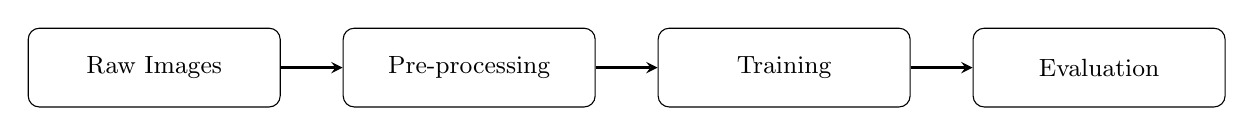
\begin{tikzpicture}[
        box/.style={rectangle, rounded corners, draw, align=center, minimum width=3.2cm, minimum height=1cm, font=\small},
        arrow/.style={->, >=stealth, thick}
    ]
        \node[box] (input) at (0,0) {Raw Images};
        \node[box] (prep) at (4,0) {Pre-processing};
        \node[box] (train) at (8,0) {Training};
        \node[box] (eval) at (12,0) {Evaluation};

        \draw[arrow] (input) -- (prep);
        \draw[arrow] (prep) -- (train);
        \draw[arrow] (train) -- (eval);
    \end{tikzpicture}
    }
    \caption{High-level processing pipeline of the handwritten digit classification system.}
    \label{fig:highlevel-pipeline}
\end{figure}

Figure~\ref{fig:highlevel-pipeline} presents the overall framework of the proposed system as a linear processing pipeline.

\textit{Raw Images} stage provides handwritten digit samples as grayscale images stored in folder structure.
These images serve as the original data source for the learning process.

\textit{Pre-processing} stage converts raw images into numerical vectors by loading images from folders, converting to grayscale, resizing to $28 \times 28$ pixels, flattening into 784-dimensional vectors, and normalizing pixel values using standardization.

\textit{Training} stage, model parameters are optimized using labeled data through supervised learning with mini-batch stochastic gradient descent, with the objective of minimizing cross-entropy loss.

\textit{Evaluation} stage measures the predictive performance of the trained model on unseen data using quantitative metrics such as accuracy and loss, along with visualization tools including confusion matrices and prediction samples.
